\tikzset{every picture/.style={line width=0.75pt}} %set default line width to 0.75pt        

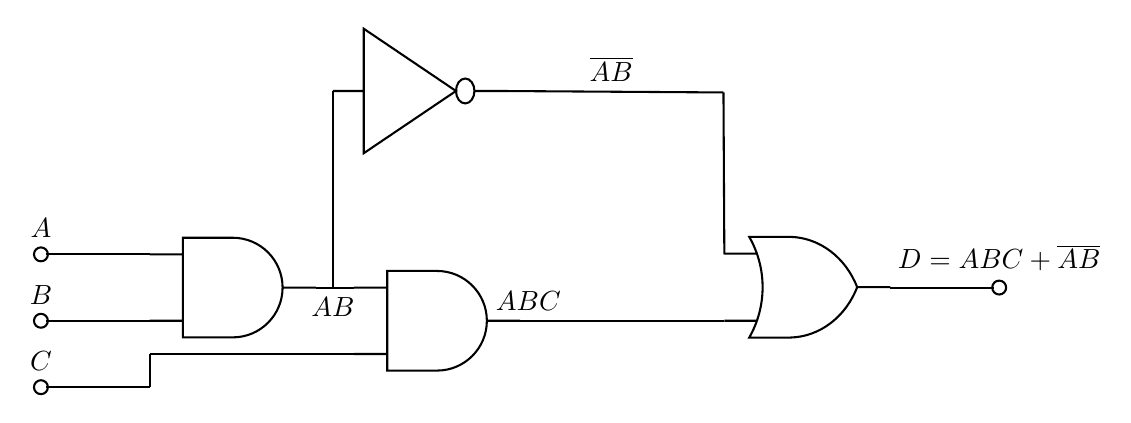
\begin{tikzpicture}[x=0.75pt,y=0.75pt,yscale=-1,xscale=1]
%uncomment if require: \path (0,393); %set diagram left start at 0, and has height of 393

%Straight Lines [id:da23815456210484298] 
\draw    (131.71,157) -- (81.64,157) ;
\draw [shift={(79.29,157)}, rotate = 180] [color={rgb, 255:red, 0; green, 0; blue, 0 }  ][line width=0.75]      (0, 0) circle [x radius= 3.35, y radius= 3.35]   ;
%Straight Lines [id:da04610179645106571] 
\draw    (131.71,189) -- (81.64,189) ;
\draw [shift={(79.29,189)}, rotate = 180] [color={rgb, 255:red, 0; green, 0; blue, 0 }  ][line width=0.75]      (0, 0) circle [x radius= 3.35, y radius= 3.35]   ;
%Straight Lines [id:da7638407091081825] 
\draw    (131.71,221) -- (81.64,221) ;
\draw [shift={(79.29,221)}, rotate = 180] [color={rgb, 255:red, 0; green, 0; blue, 0 }  ][line width=0.75]      (0, 0) circle [x radius= 3.35, y radius= 3.35]   ;
%Shape: And Gate [id:dp1564557077664277] 
\draw   (147.71,149) -- (171.71,149) .. controls (184.96,149) and (195.71,159.75) .. (195.71,173) .. controls (195.71,186.25) and (184.96,197) .. (171.71,197) -- (147.71,197) -- (147.71,149) -- cycle (131.71,157) -- (147.71,157) (131.71,189) -- (147.71,189) (195.71,173) -- (211.71,173) ;
%Shape: And Gate [id:dp07355261068451113] 
\draw   (246.13,165) -- (270.13,165) .. controls (283.38,165) and (294.13,175.75) .. (294.13,189) .. controls (294.13,202.25) and (283.38,213) .. (270.13,213) -- (246.13,213) -- (246.13,165) -- cycle (230.13,173) -- (246.13,173) (230.13,205) -- (246.13,205) (294.13,189) -- (310.13,189) ;
%Straight Lines [id:da4661863224212748] 
\draw    (230.13,173) -- (211.71,173) ;
%Straight Lines [id:da3821485817926048] 
\draw    (230.13,205) -- (131.71,205) ;
%Straight Lines [id:da9213385284221522] 
\draw    (131.71,221) -- (131.71,205) ;
%Straight Lines [id:da9899457357378714] 
\draw    (408.55,189) -- (310.13,189) ;
%Straight Lines [id:da2621263792990446] 
\draw    (408.13,79) -- (408.55,157) ;
%Straight Lines [id:da026515041729731847] 
\draw    (488.55,173) -- (538.62,173) ;
\draw [shift={(540.97,173)}, rotate = 0] [color={rgb, 255:red, 0; green, 0; blue, 0 }  ][line width=0.75]      (0, 0) circle [x radius= 3.35, y radius= 3.35]   ;
%Straight Lines [id:da3970001006084427] 
\draw    (220,78.29) -- (220,172.71) ;
%Shape: Not/Inverter Gate [id:dp48812914811132324] 
\draw   (234.81,48.29) -- (279.26,78.29) -- (234.81,108.29) -- (234.81,48.29) -- cycle (220,78.29) -- (234.81,78.29) (288.15,78.29) -- (300,78.29) (279.26,78.29) .. controls (279.26,74.98) and (281.25,72.29) .. (283.7,72.29) .. controls (286.16,72.29) and (288.15,74.98) .. (288.15,78.29) .. controls (288.15,81.6) and (286.16,84.29) .. (283.7,84.29) .. controls (281.25,84.29) and (279.26,81.6) .. (279.26,78.29) -- cycle ;
%Straight Lines [id:da25799347375209314] 
\draw    (408.13,79) -- (300,78.29) ;
%Shape: Or Gate [id:dp8158339008286285] 
\draw   (420.55,148.58) -- (440.55,148.58) .. controls (454.51,149.02) and (466.98,158.47) .. (472.55,172.83) .. controls (466.98,187.2) and (454.51,196.65) .. (440.55,197.08) -- (420.55,197.08) .. controls (429.13,182.08) and (429.13,163.59) .. (420.55,148.58) -- cycle (408.55,156.67) -- (424.55,156.67) (408.55,189) -- (424.55,189) (472.55,172.83) -- (488.55,172.83) ;

% Text Node
\draw (79.29,150.6) node [anchor=south] [inner sep=0.75pt]    {$A$};
% Text Node
\draw (79.29,182.6) node [anchor=south] [inner sep=0.75pt]    {$B$};
% Text Node
\draw (79.29,214.6) node [anchor=south] [inner sep=0.75pt]    {$C$};
% Text Node
\draw (220,176.11) node [anchor=north] [inner sep=0.75pt]    {$AB$};
% Text Node
\draw (314.13,185.6) node [anchor=south] [inner sep=0.75pt]    {$ABC$};
% Text Node
\draw (540.97,166.6) node [anchor=south] [inner sep=0.75pt]    {$D=ABC+\overline{AB}$};
% Text Node
\draw (354.07,75.24) node [anchor=south] [inner sep=0.75pt]    {$\overline{AB}$};


\end{tikzpicture}
